\documentclass[11pt,letterpaper]{exam}
\usepackage[utf8]{inputenc}
\usepackage[spanish]{babel}
\usepackage{graphicx}
\usepackage{tabularx}
\usepackage[absolute]{textpos} % Para poner una imagen en posiciones arbitrarias
\usepackage{multirow}
\usepackage{float}
\usepackage{hyperref}
%\decimalpoint

\begin{document}
\begin{center}
{\Large Métodos Computacionales} \\
\textsc{Tarea 2}\\
{\large Ana María Bello Peña}\\
201613035\\
Julio - 2019\\
\end{center}

\noindent
\section{Transformada de Fourier: Im\'agenes H\'ibridas.}
\begin{center}
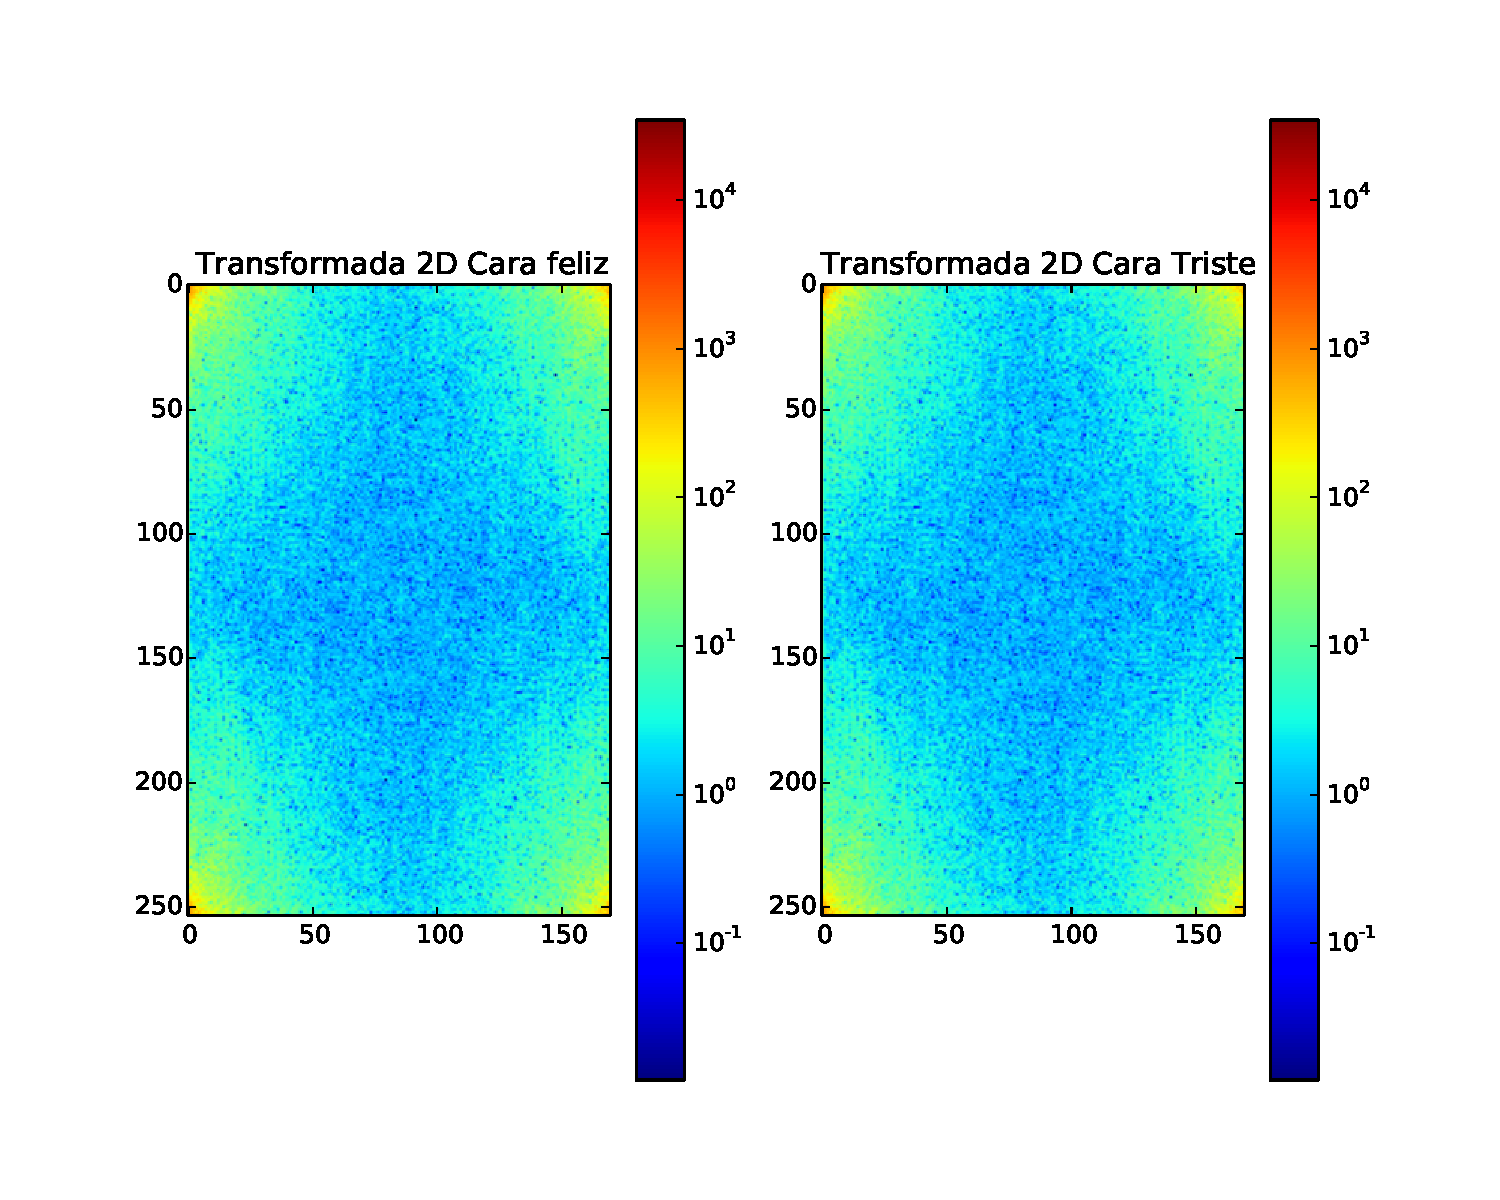
\includegraphics[width=16.cm]{FFtIm.pdf}
\textbf{Figura 1:}{ Espectros de Fourier de las im\'agenes.'}
\end{center}

{Las frecuencias van de un intervalo de $10^{-1}$ a $10^{3}$, los bordes poseen mayores frecuencias con respecto al centro, por ende si se realiza filtrado pasa bajos o pasa altos, las im\'agenes se ver\'a afectado el borde en el caso de pasa bajps y el centro en el caso de pasa altos.}

\begin{center}
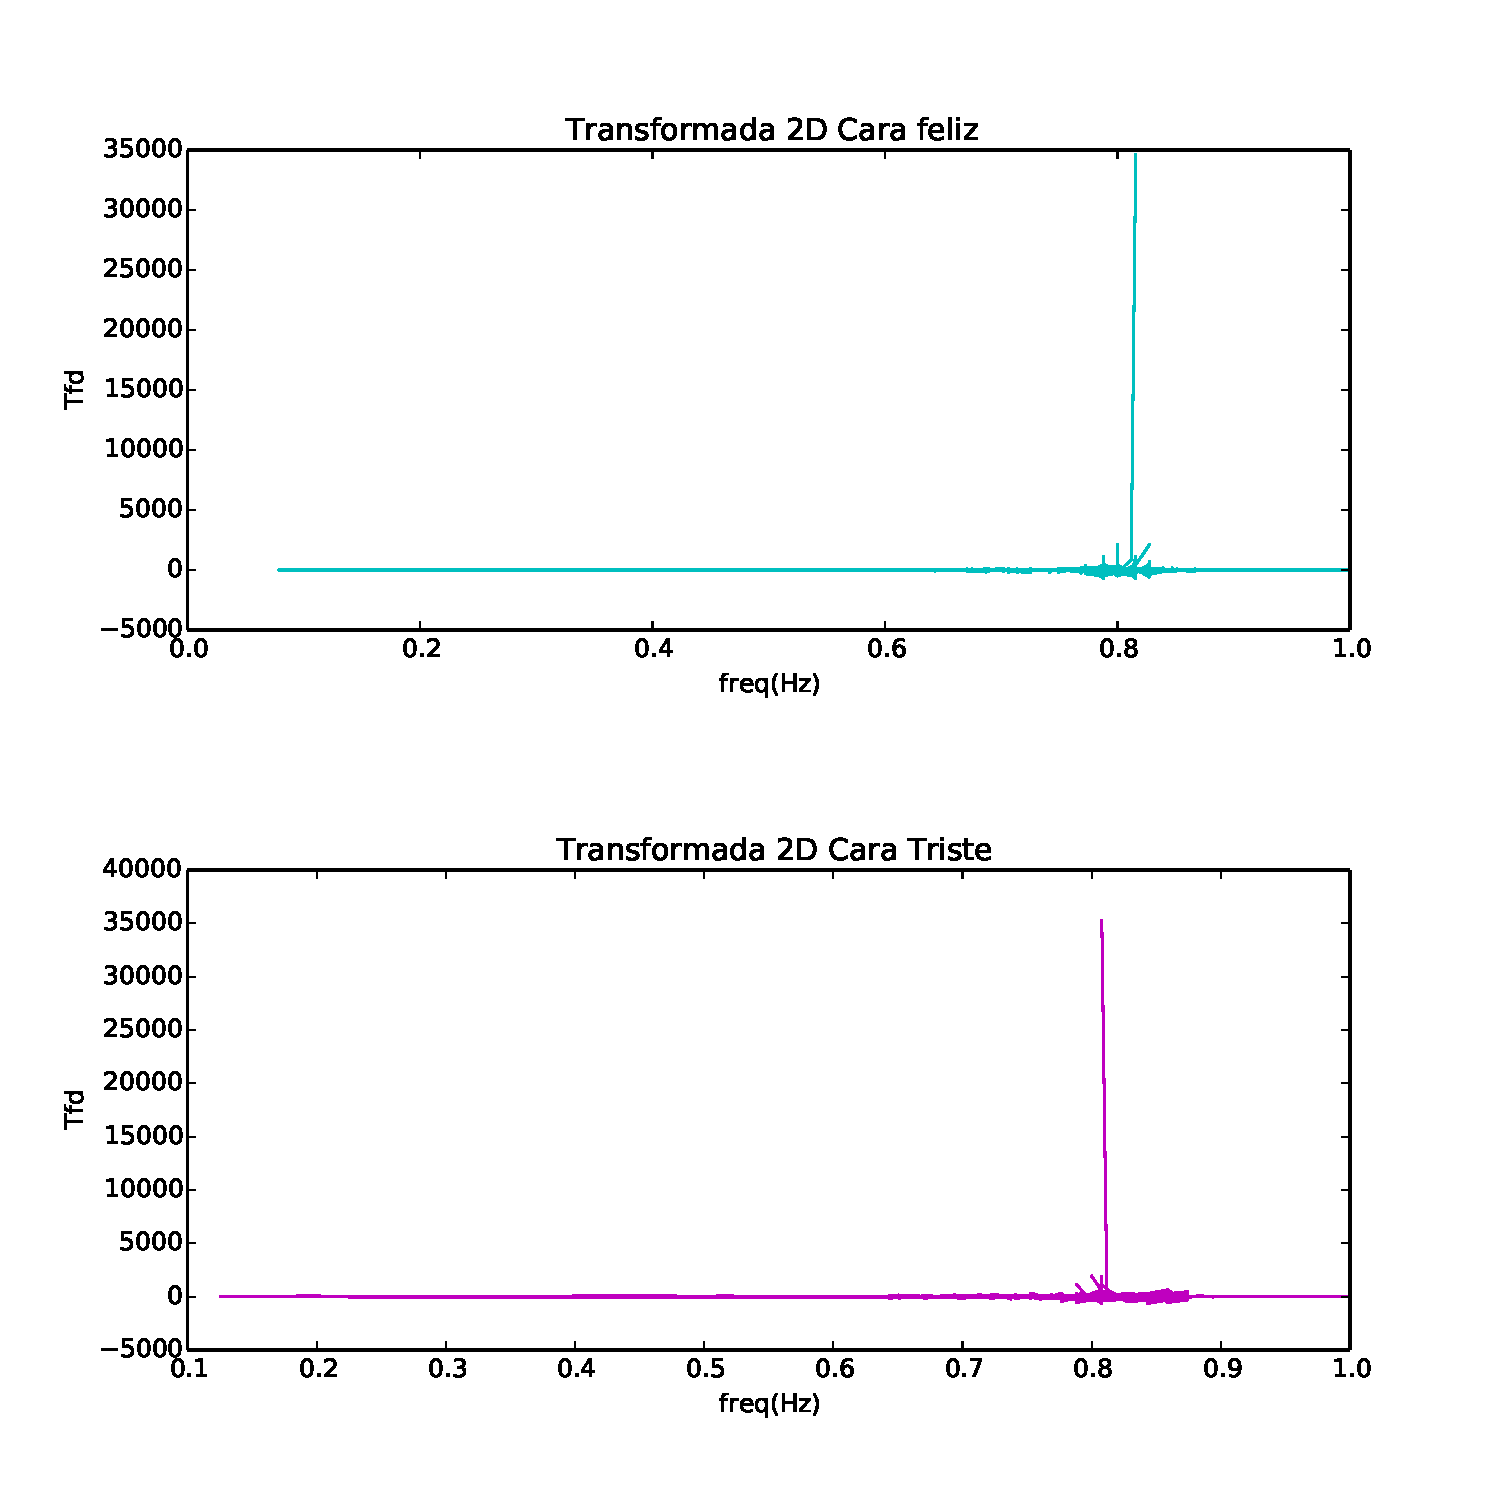
\includegraphics[width=16.cm]{FFt.pdf}
\textbf{Figura 2:}{ Transformada de Fourier 2D de las im\'agenes.}
\end{center}

{En esta figura se gr\'afica las transformada Fourier 2D en funci\'on de las frecuencias, se puede observar que ambas im\'agenes poseen un pico con el valor de Transformada de 35000, la cual puede ser considerada una frecuencia principal, se observa que hay una concentración frecuencias mayores a cero dentro del intervalo 0.7-0.9 Hz.	
}

\begin{center}
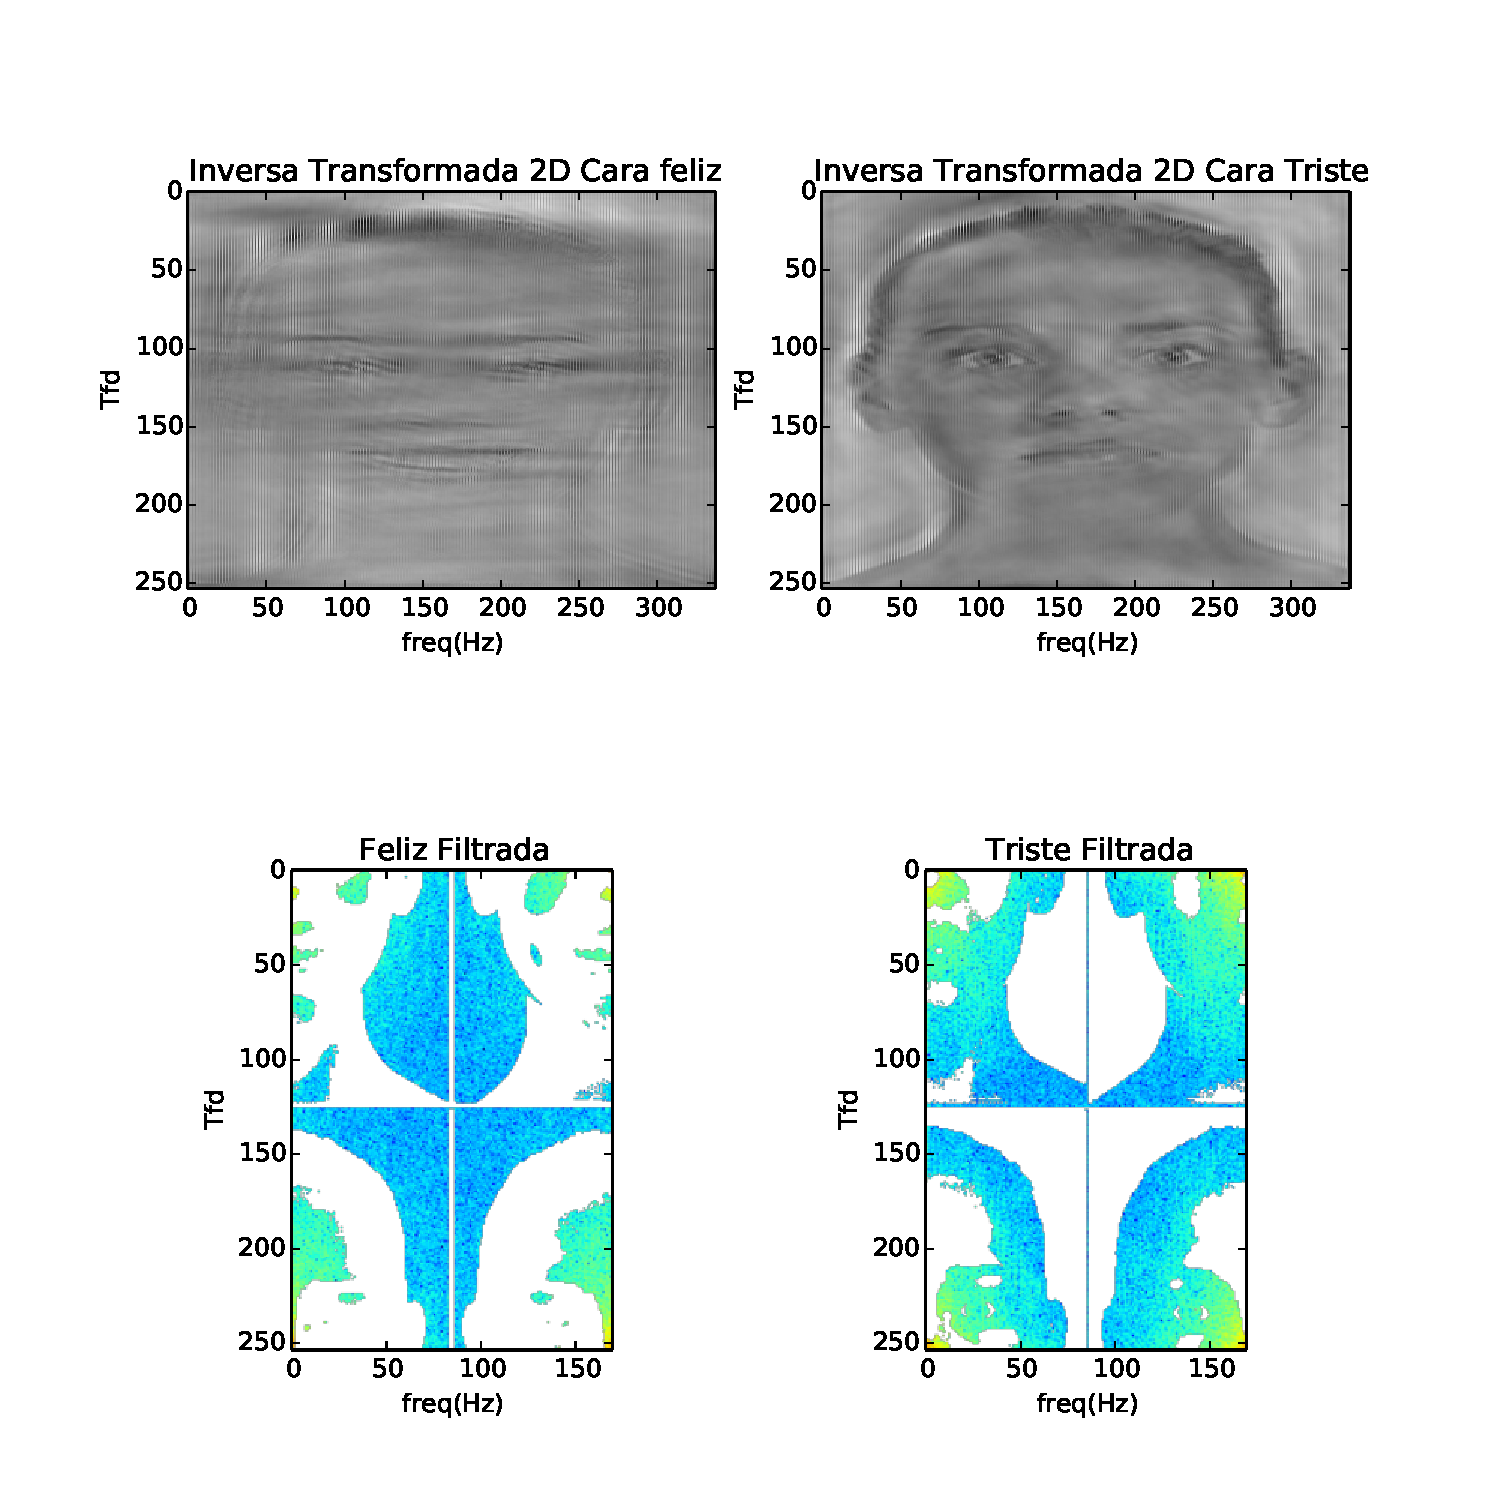
\includegraphics[width=16.cm]{ImProceso.pdf}
\textbf{Figura 3:}{ Proceso de filtrado de im\'agenes.}
\end{center}

{Para la realizaci\'on de la im\'agen h\'ibrida se realizar\'on filtros a las im\'agenes con el fin de eliminar las frecuencias bajas y altas de las mismas. El objetivo de el filtrado es eliminar a una foto los bordes para desenfocar con respecto a la otra. De este modo se pudiera observar seria de cerca y feliz desde lejos. Para realizar im\'agenes hibridas se necesitan m\'as filtros gaussianos y convoluci\'on para lograr una buena definici\'on. En este ejercicio se opt\'o por filtrar las TFD en 2D para obtener un resultado parecido. En los dos primeros subplots se ven las im\'agenes con la inversa de la TFD 2D aplicada para poder observar la imagen y en los otros subplots se grafic\'o la parte real de la transformada.}

\begin{center}
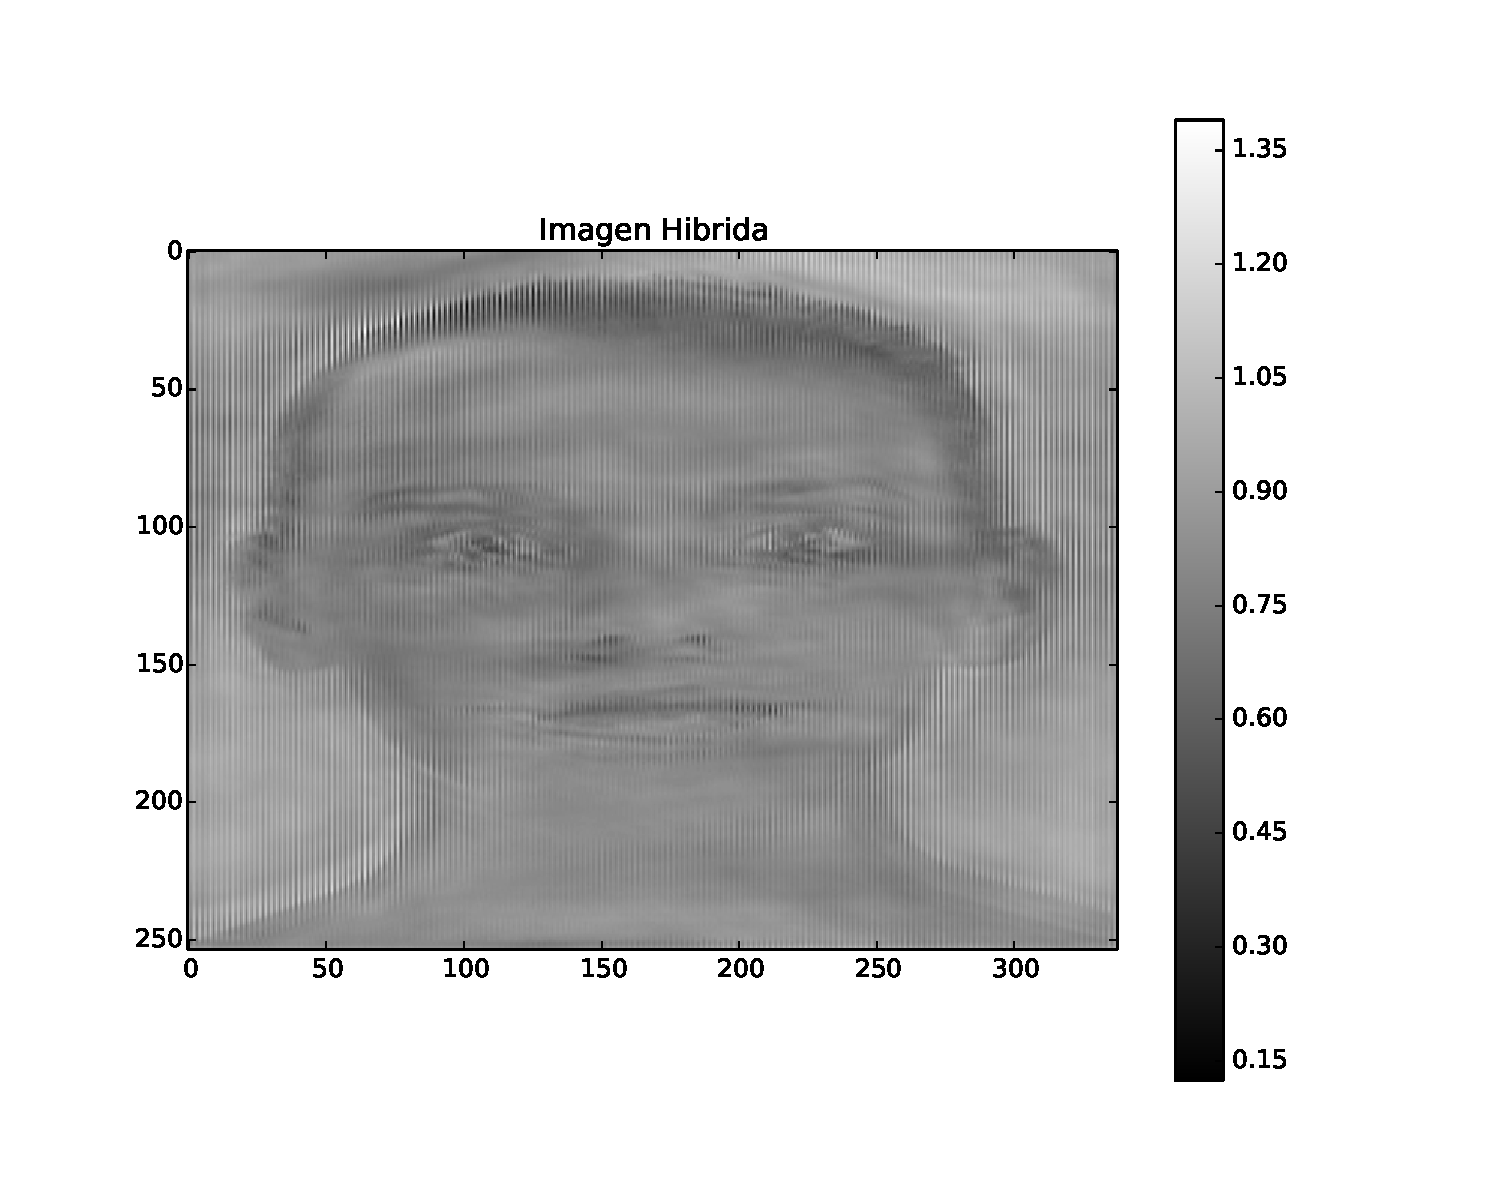
\includegraphics[width=16.cm]{ImHybrid.pdf}
\textbf{Figura 4:}{ Imagen H\'ibrida.}
\end{center}

{ Finalmente, se obtuvo este resultado aplicando los filtros de pasa bajos y pasa altos y sumando las partes reales de las transformadas inversas de ambas im\'agenes. El resultado no fue satisfactorio gracias a que hay un ruido periodico en la im\'agen. Este ruido se intento eliminar sumando valores de coseno, a partir de la gu\'ia del curso Filtering in the Frequency Domain de coursera.}

\noindent
\section{Ejercicio 2: Comparaci\'on de los distintos m\'etodos de soluci\'on de ecuaciones diferenciales ordinarias: Caso masa orbitando alrededor de otra.}

\begin{center}
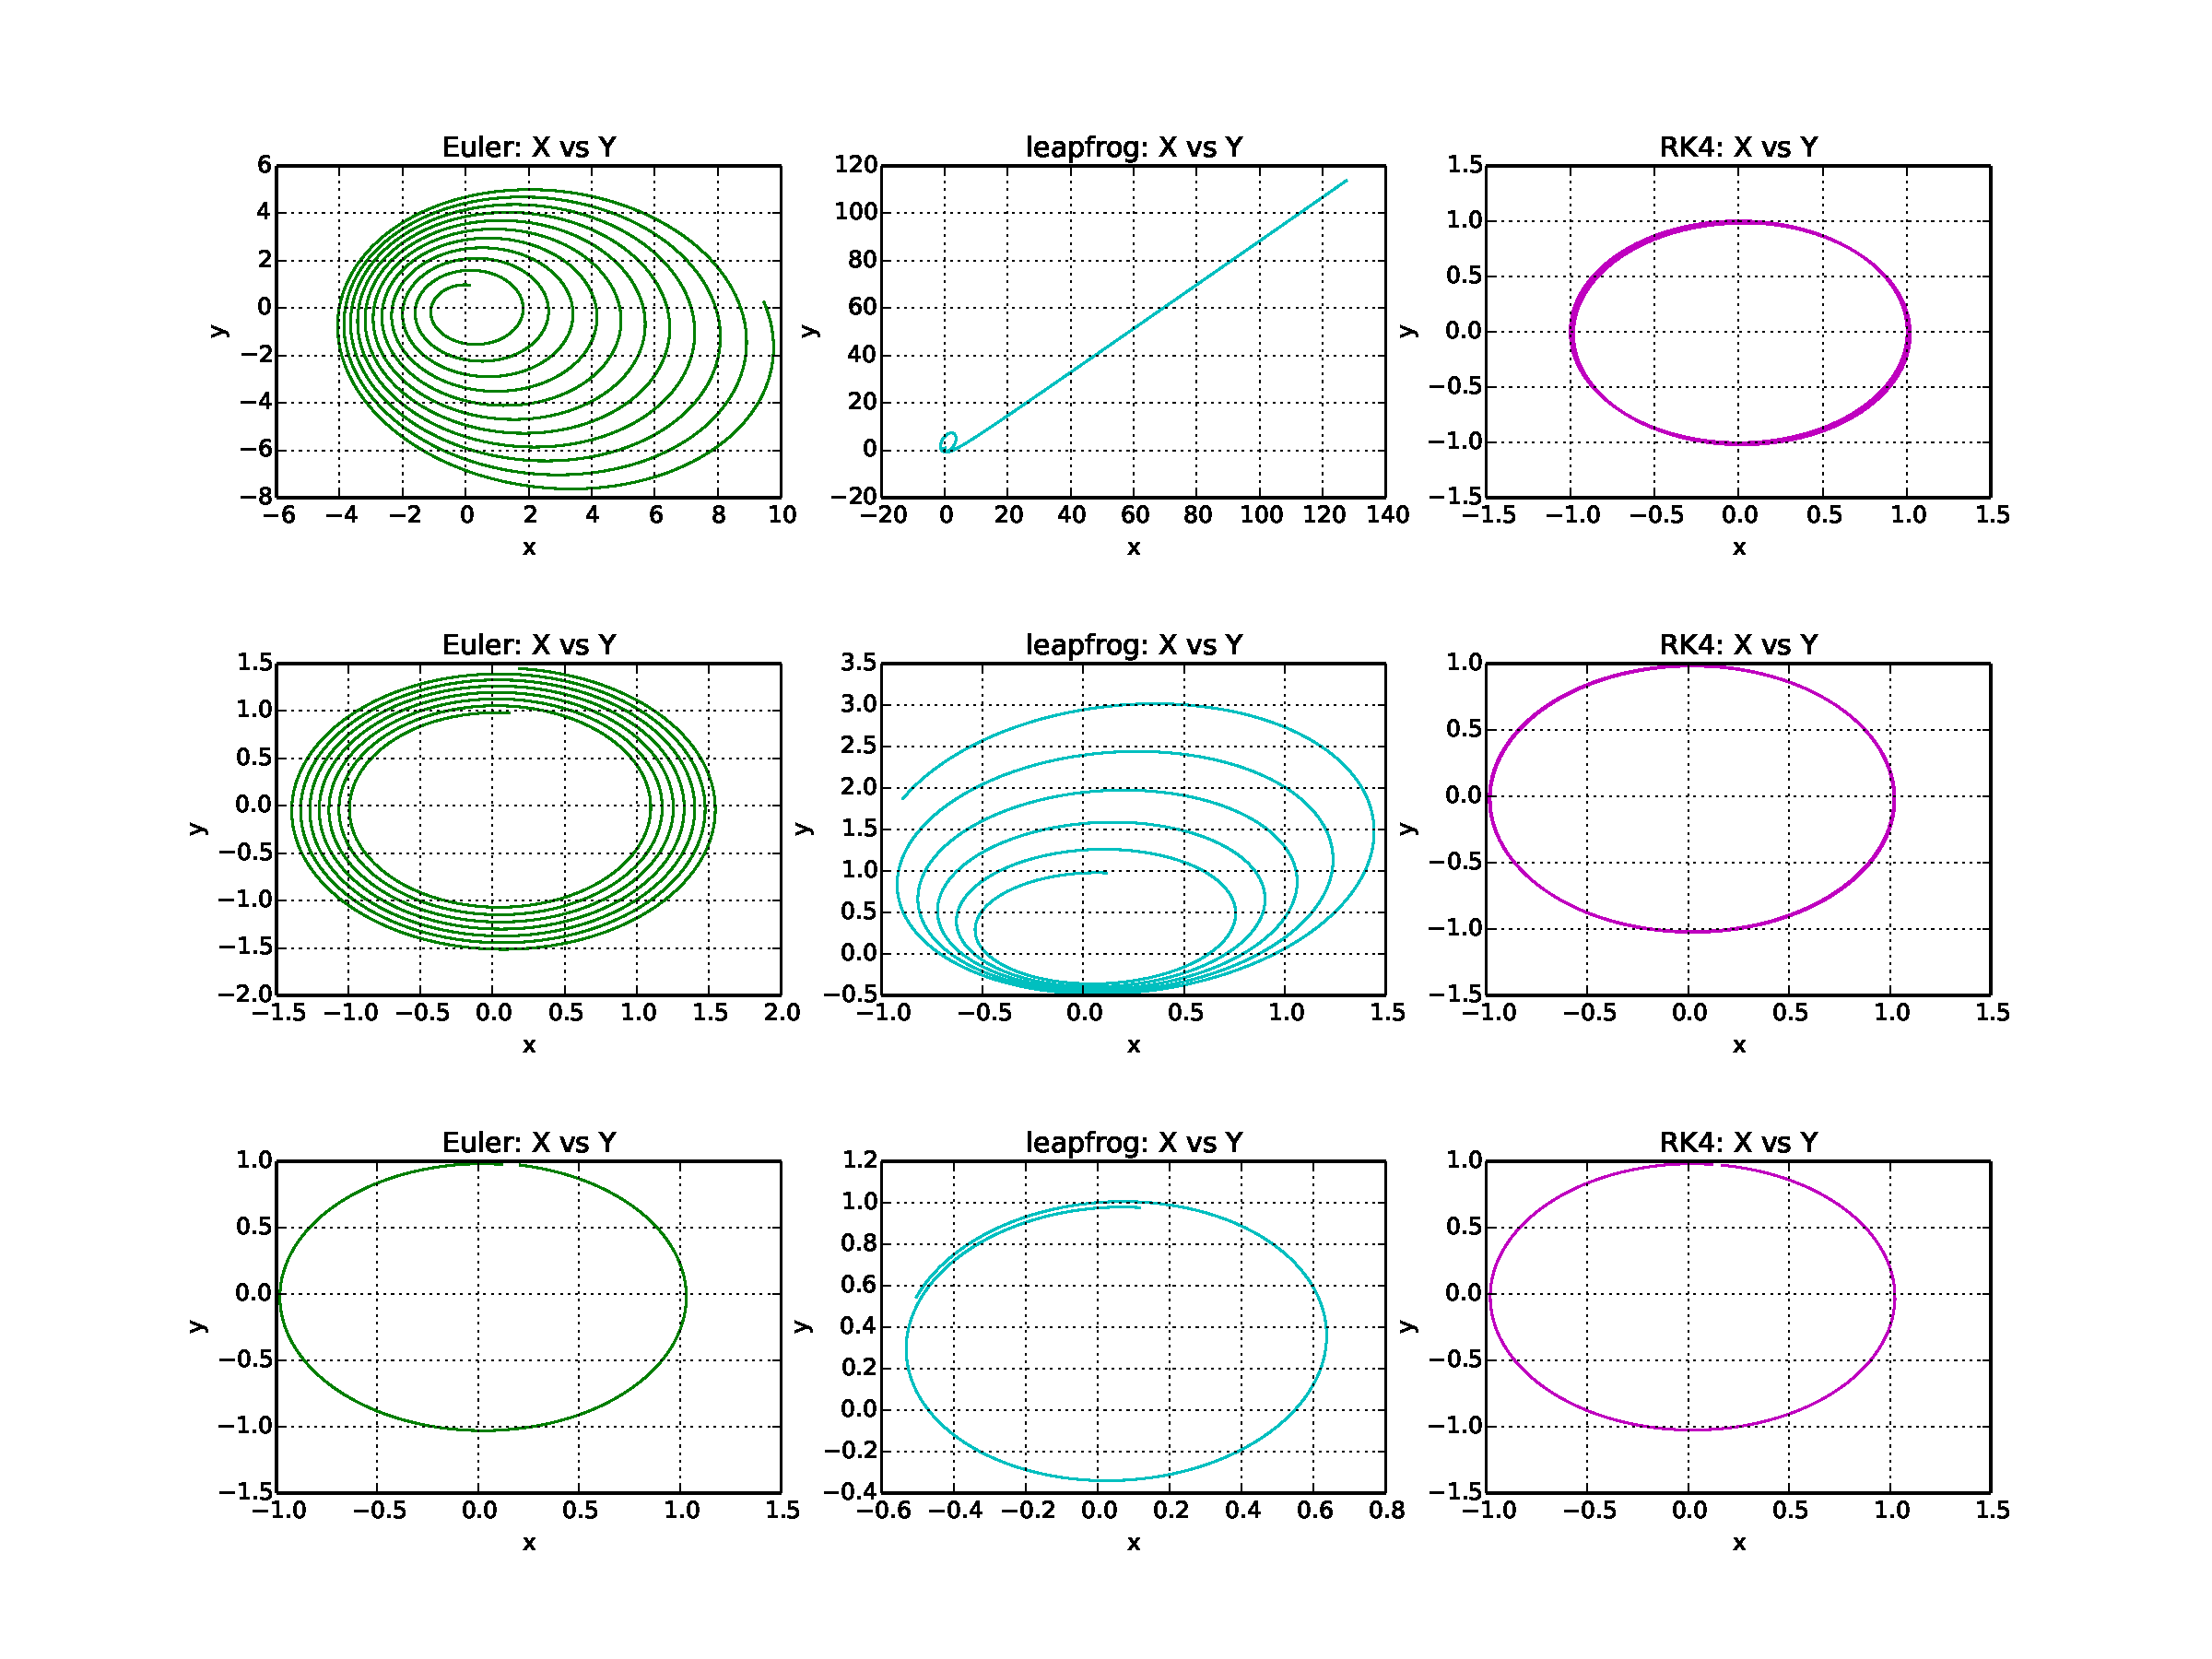
\includegraphics[width=16.cm]{XY_met_dt.pdf}
\textbf{Figura 5:}{  X vs Y de diferentes m\'etodos y dts.}
\end{center}

\begin{center}
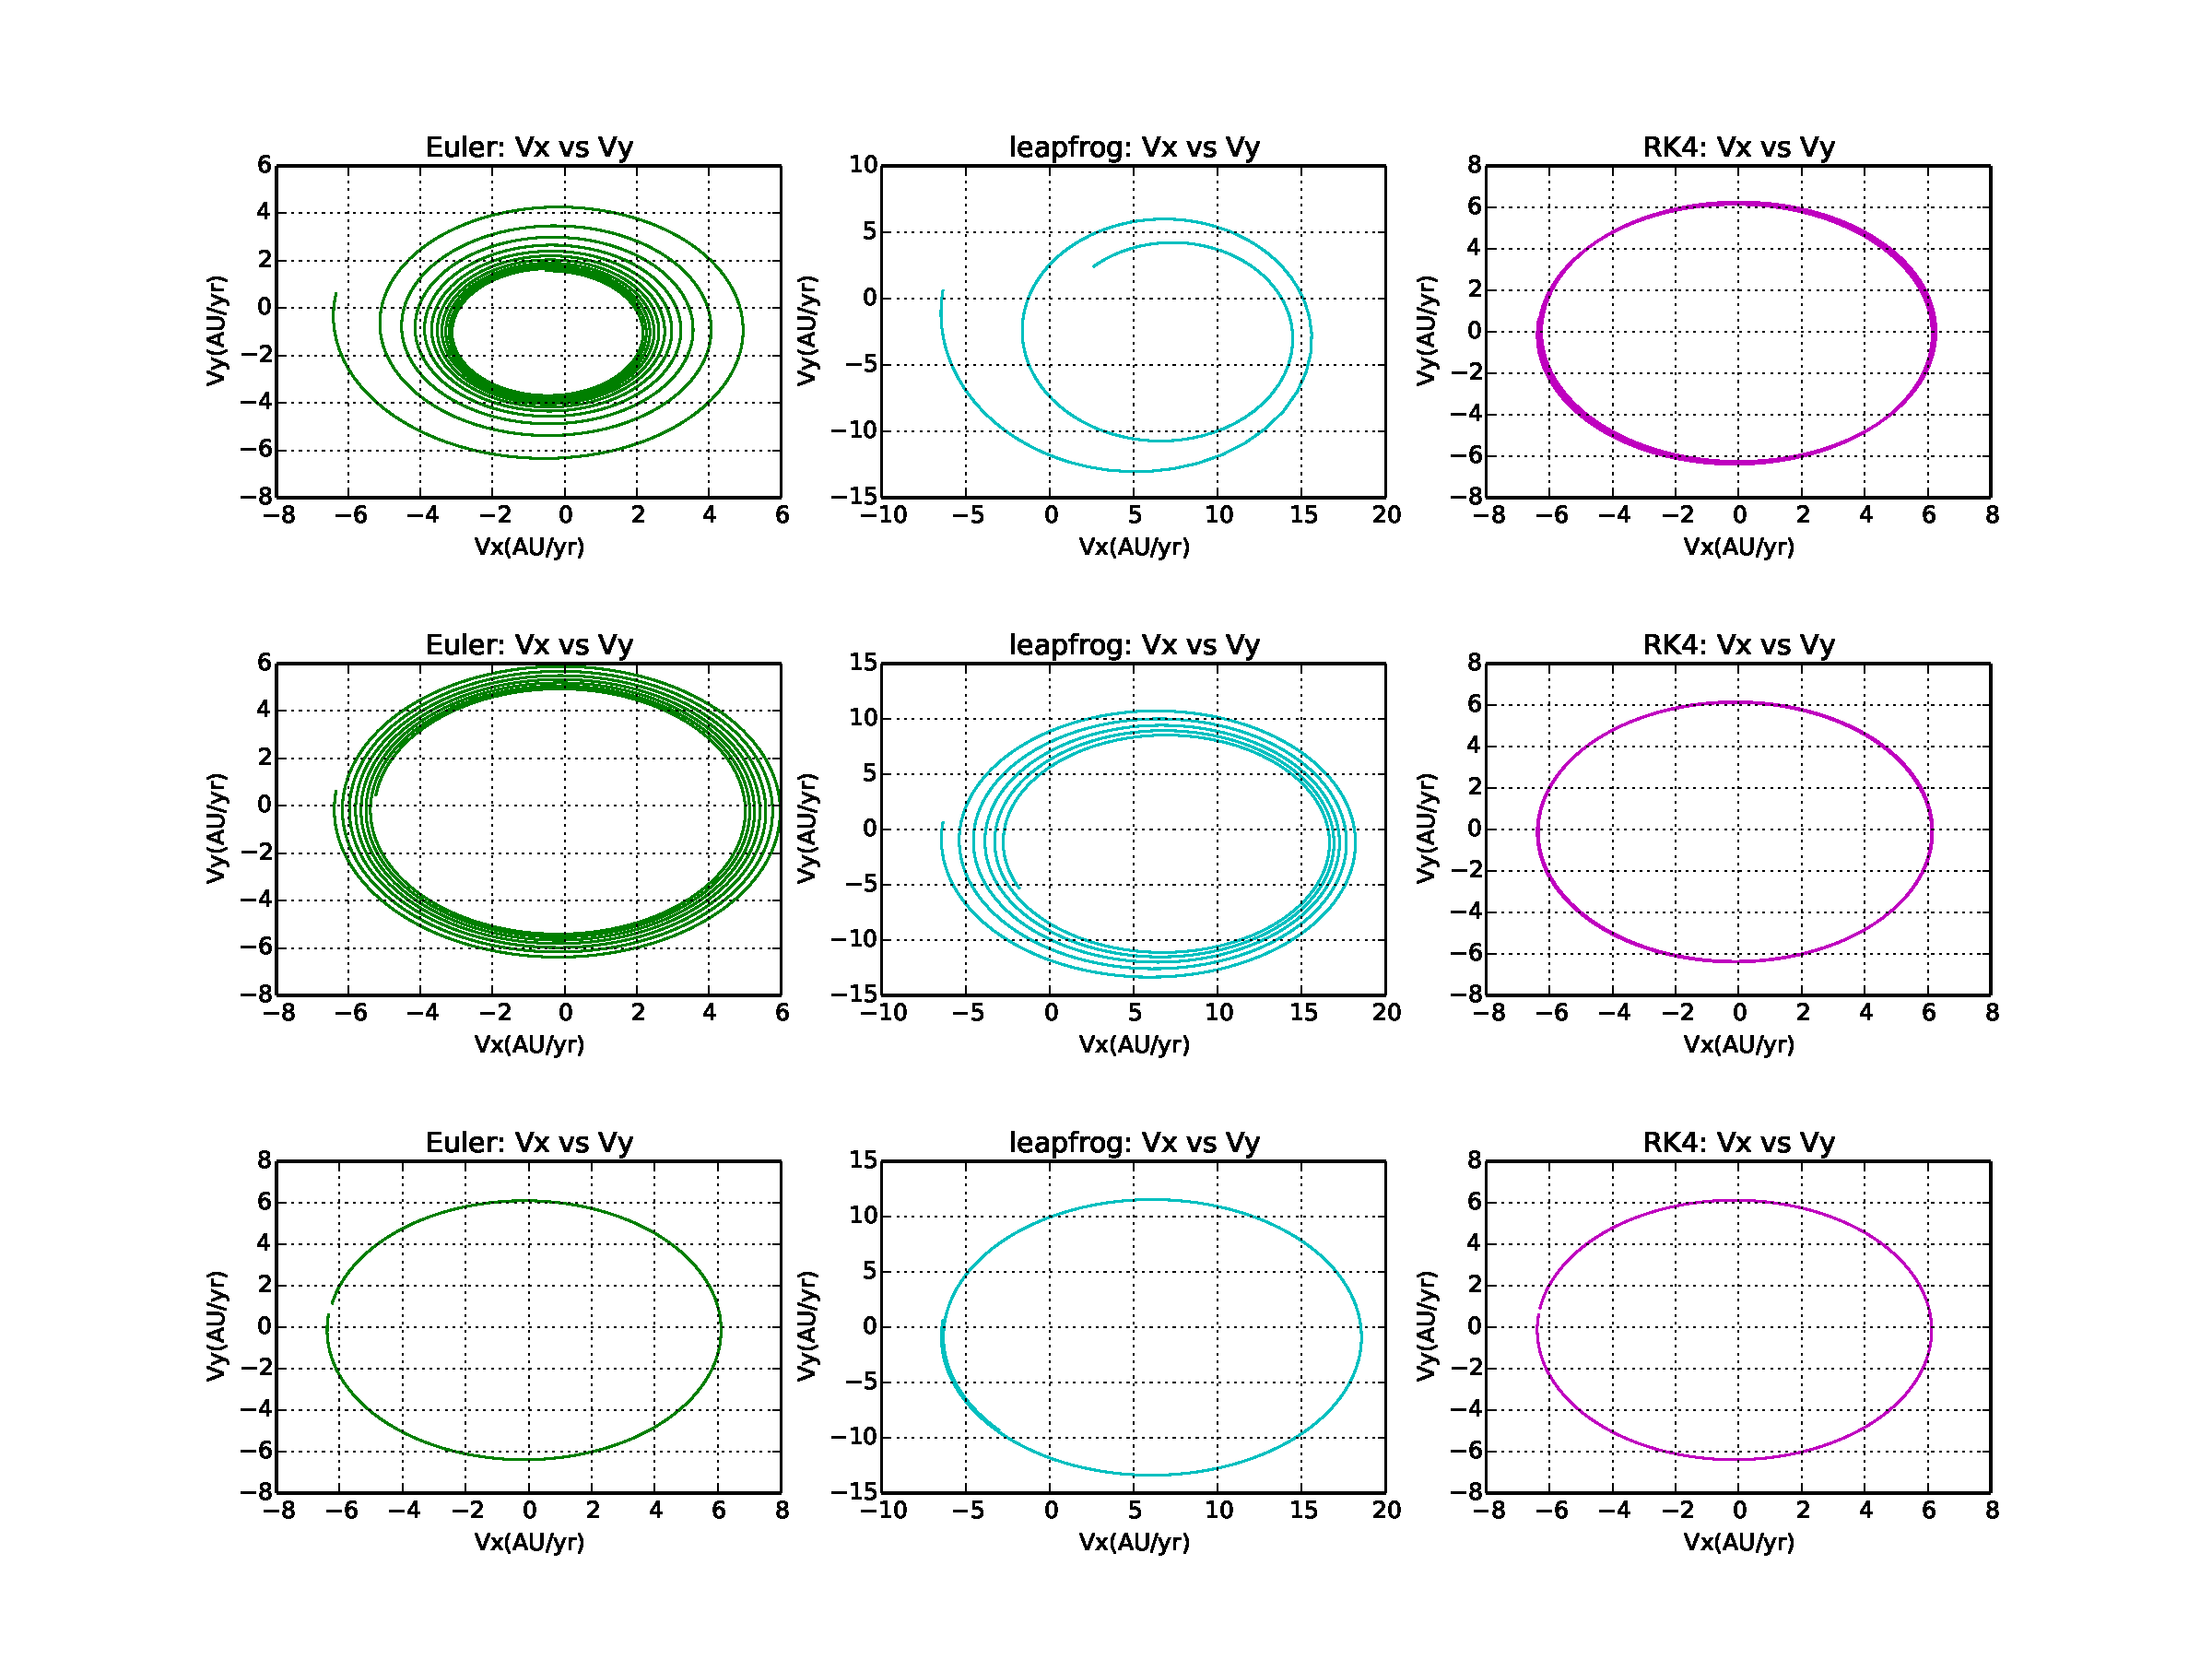
\includegraphics[width=16.cm]{VxVy_met_dt.pdf}
\textbf{Figura 6:}{  VX vs VY de diferentes m\'etodos y dts.}
\end{center}

\begin{center}
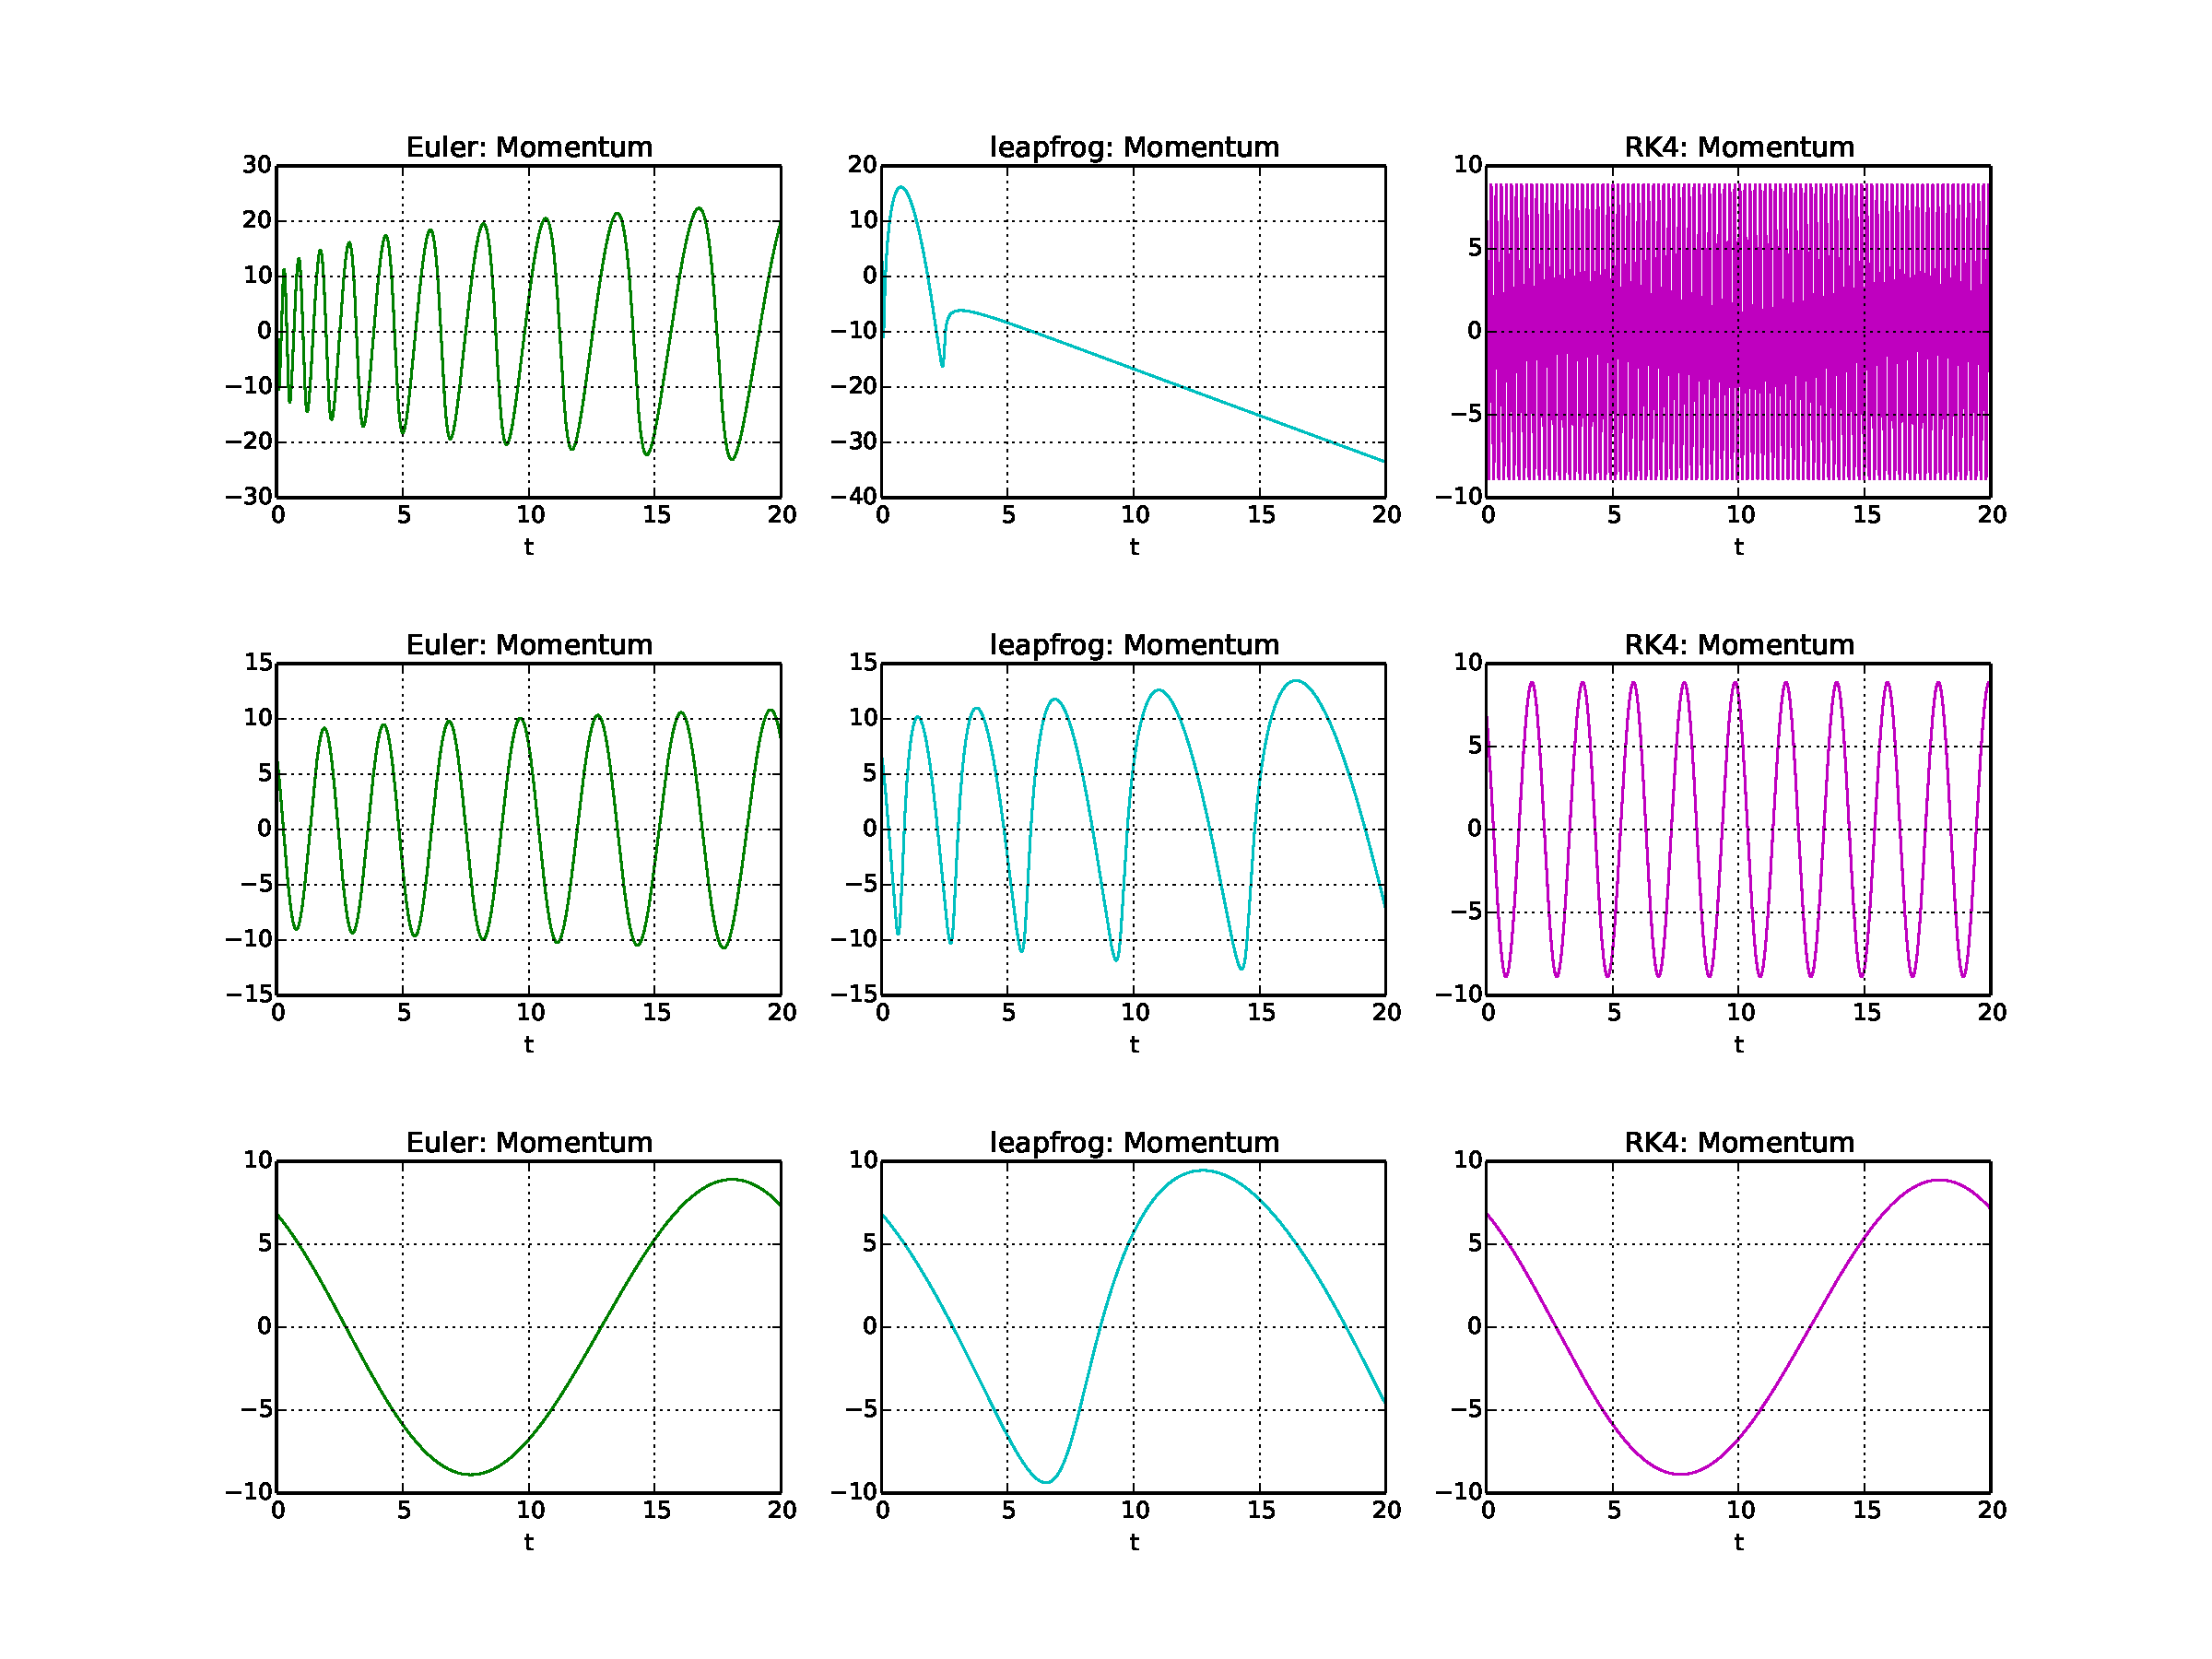
\includegraphics[width=16.cm]{Mome_met_dt.pdf}
\textbf{Figura 7:}{  Momentum de diferentes m\'etodos y dts.}
\end{center}

\begin{center}
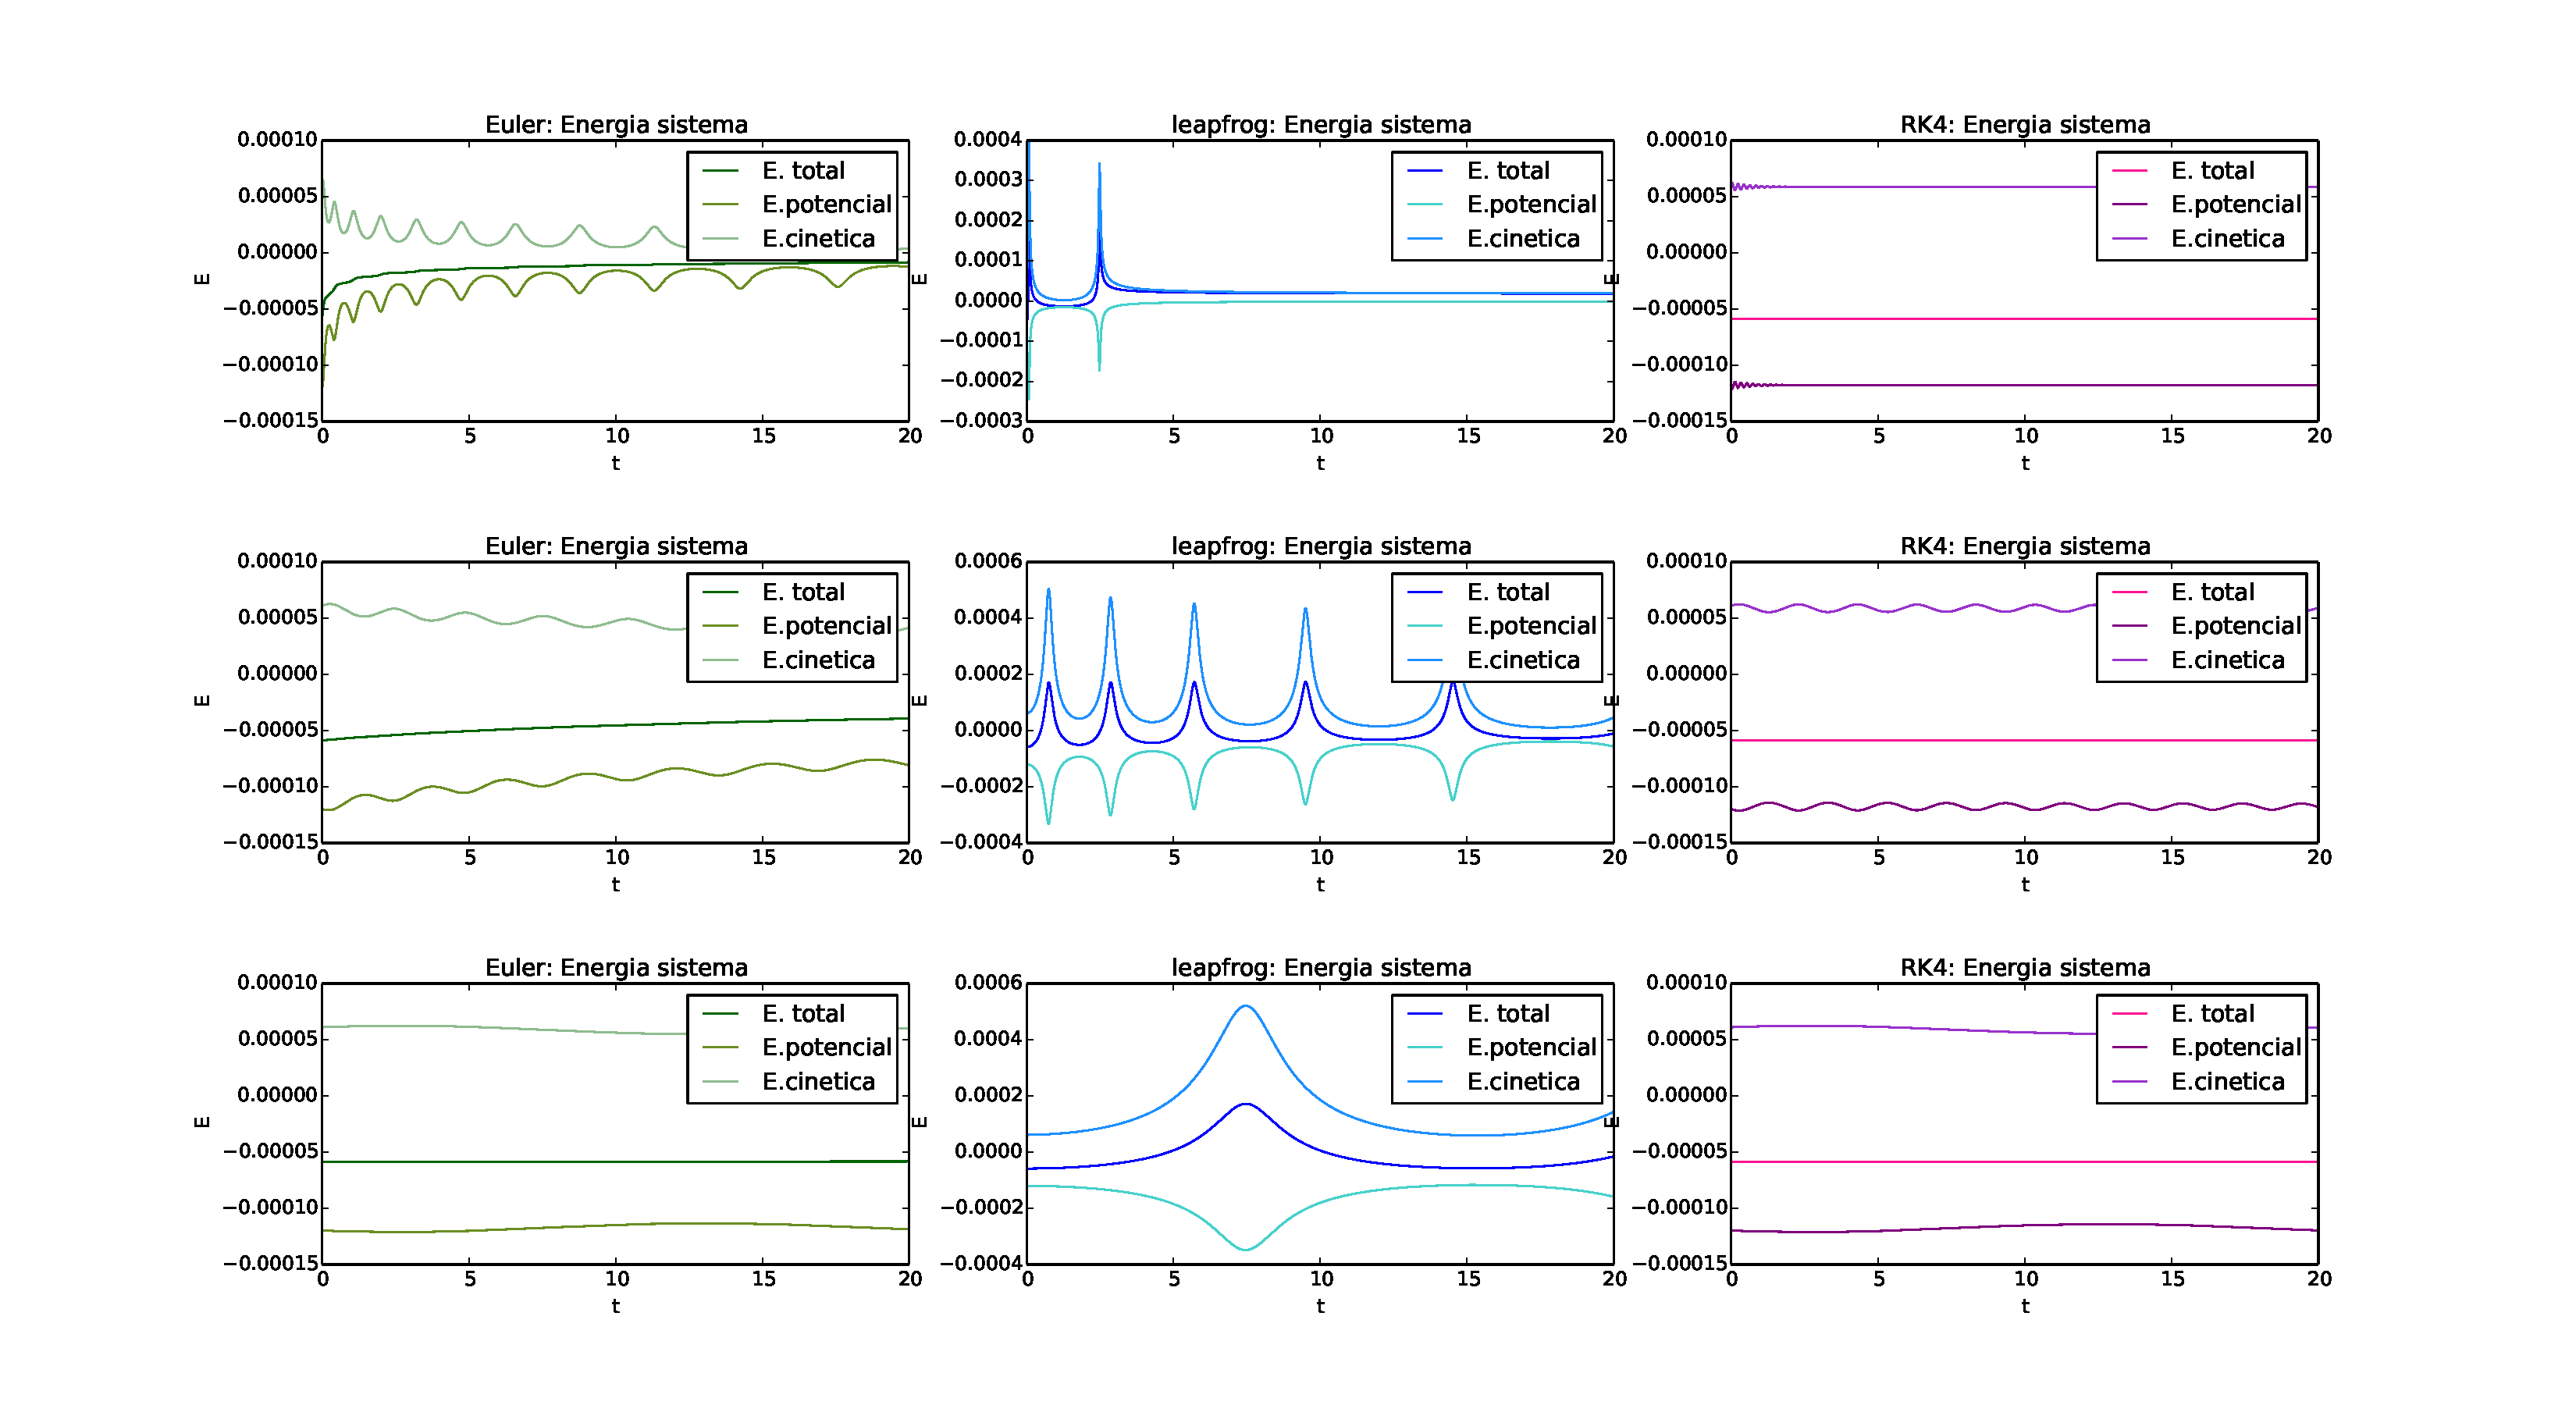
\includegraphics[width=16.cm]{Ener_met_dt.pdf}
\textbf{Figura 8:}{  Energ\'ia total del sistema de diferentes m\'etodos y dts.}
\end{center}

\begin{center}
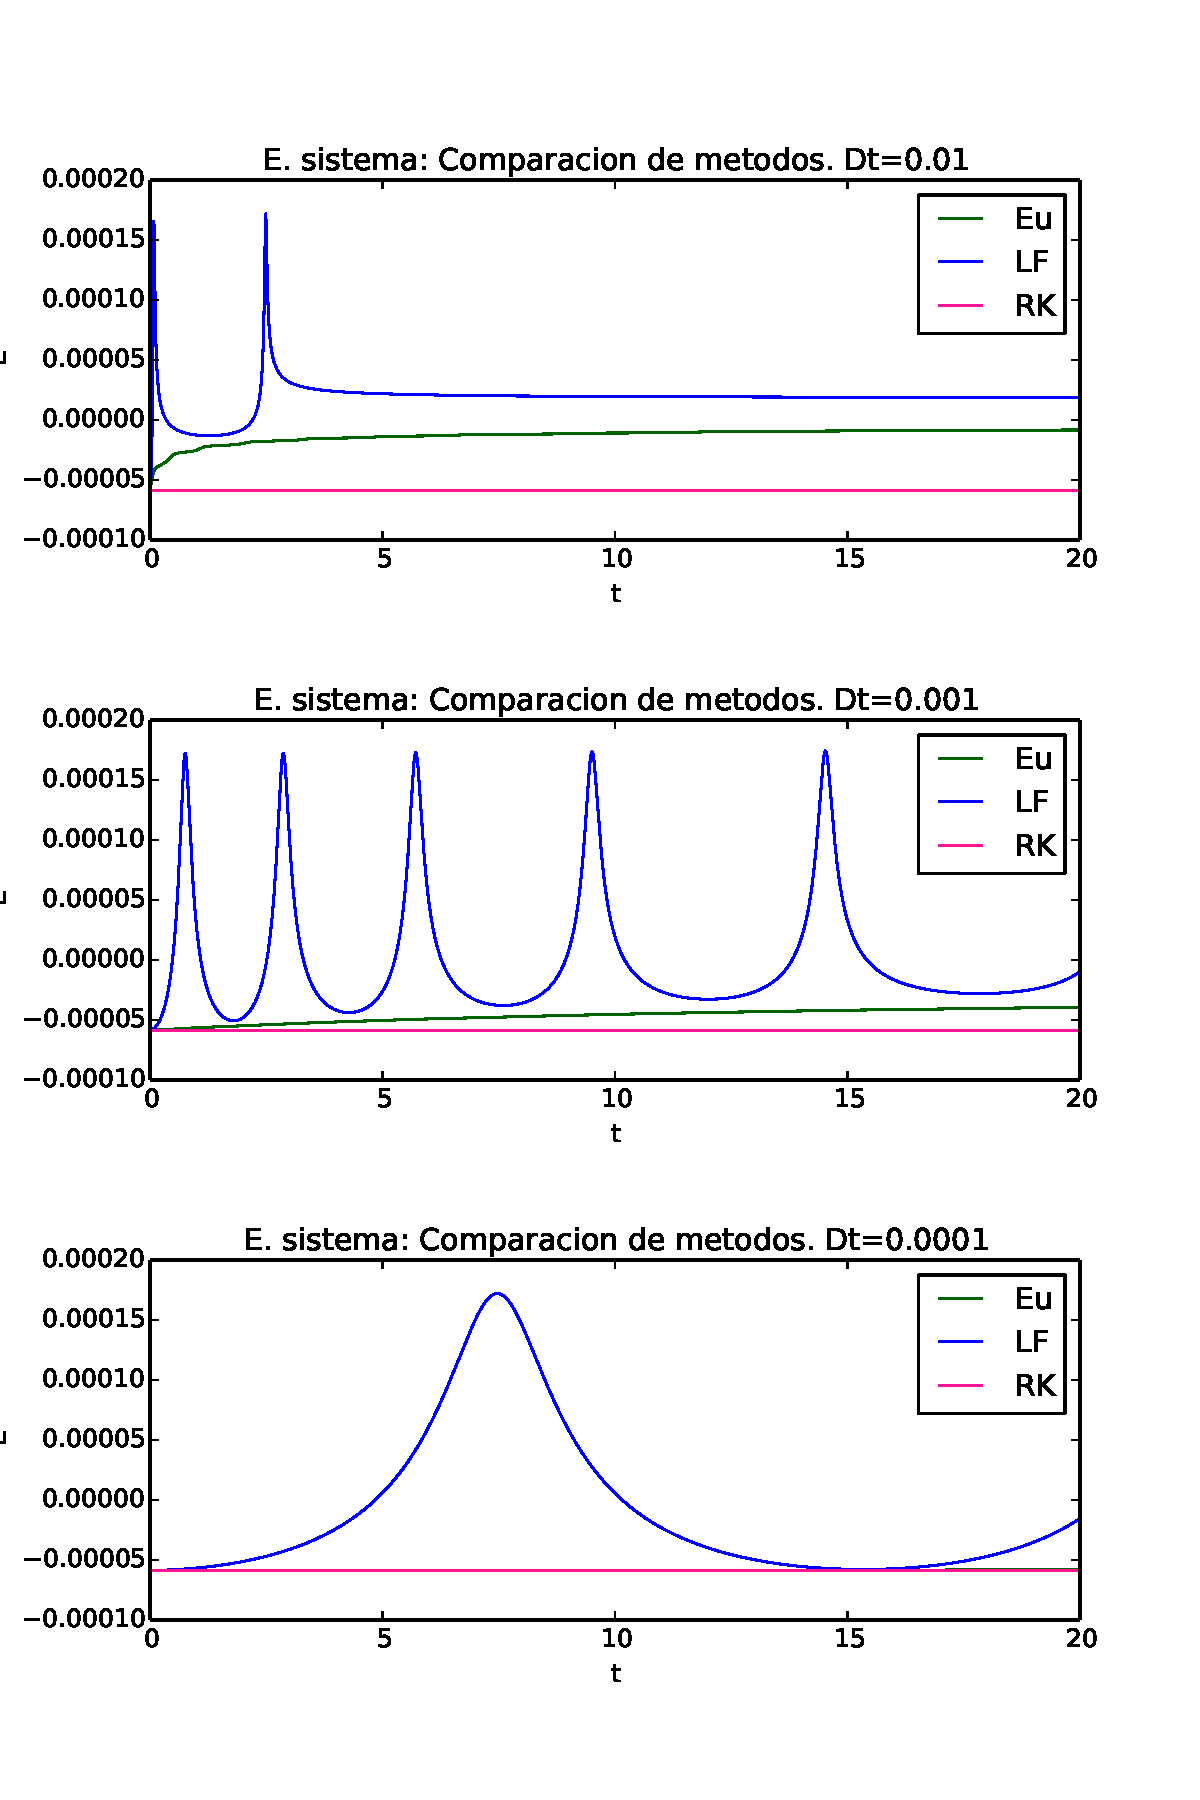
\includegraphics[width=16.cm]{Enertotal_met_dt.pdf}
\textbf{Figura 9:}{  Energ\'ias total del sistema comparaci\'on de m\'etodos y dts.}
\end{center}

\end{document}